\newpage
\section{Implementation}
The hardware description of the implemented game pong is divided into six modules. Firstly the video controller, which implements the VGA respectively HDMI interface, provides the functionality to display the video output on a monitor. Two modules generate the inputs for the movement of the paddles. The right paddle is controlled by the debounced up and down buttons of the board and the right paddle is controlled by the computer opponent. Additionally the image generator creates all required objects like the ball and paddles as well as their movement. Furthermore the match controller manages the interactions between the objects and the state of the match itself. Lastly the audio output is created by the sound generator module.
	\subsection{Video Controller}
    The video controller provides an interface for the image generator so objects can easily be displayed on a monitor. Thereby it makes the coordinates of the current pixel available and hides all additional requirements of the protocol like timing. The point of origin of the pixel matrix is located at the top left corner of the monitor. Because our group has access to the Atlys Spartan-6 board with HDMI connector as well as the Nexys 4 board with VGA connector, we decided to implement a video controller for both protocols, so the remaining modules could be implemented using both boards. The main focus was laid on the above mentioned uniform interface for the image generator so the remaining development is independent of the used video controller.
        \subsubsection{VGA Controller}
        \subsubsection{HDMI Controller}
    \subsection{Debouncer}
    \subsection{Computer Opponent}
    \subsection{Image Generator}
    
  %this figure was redundant, therefore it has been removed
%	\begin{figure}[here]
%		\centering
%		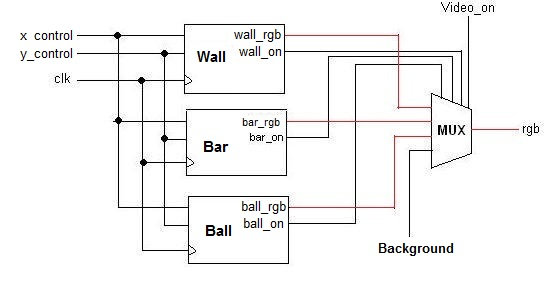
\includegraphics[scale=0.7]{images/img_gen.jpg}
%		\caption{Schematic of the Image Generator}
%		\label{img_gen}
%	\end{figure}
        The Image Generator takes inputs from the players and outputs the video that can be displayed through the HDMI interface of the Atlys board. The panels shown in figure \ref{ball_wall_panel} are submodules of the module \texttt{image\_generator\_c}.
		This module calculates the movement of the ball and movement the two panels that are controlled by the players. 
		
		The movement of the ball is done by the \texttt{ball\_c} module. (see next Section for more details on implementation).
		After a well determined time frame, the ball's movement direction is determined and the next \texttt{x\_pos} and \texttt{y\_pos} are either incremented or decremented. 
		
		The module \texttt{panel\_c} determines the y-coordinate of on panel based on the player input. For instance, pressing \texttt{btn\_up} increments the \texttt{y\_pos} signal if the panel did not reach the top edge already. 


    \subsection{Match Controller}
    
    \newpage
    \subsection{Sound Generator}
       The Image Generator takes inputs from the players and outputs the video that can be displayed through the HDMI interface of the Atlys board. The panels shown in figure \ref{ball_wall_panel} are submodules of the module \texttt{image\_generator\_c}.
		This module calculates the movement of the ball and movement the two panels that are controlled by the players. 
		
		The movement of the ball is done by the \texttt{ball\_c} module. (see next Section for more details on implementation).
		After a well determined time frame, the ball's movement direction is determined and the next \texttt{x\_pos} and \texttt{y\_pos} are either incremented or decremented. 
		
		The module \texttt{panel\_c} determines the y-coordinate of on panel based on the player input. For instance, pressing \texttt{btn\_up} increments the \texttt{y\_pos} signal if the panel did not reach the top edge already. 


		  \subsubsection{Sound Generator}
				In order to generate sound, we used the on board LM4550 chip. Figure \ref{snd_gen} the block diagram of the sound generator. This module takes in the sound events from the Match Controller module (i.e when sound generation should take place), reads a sound effect from a ROM and sends it to the LM4550 chip that in turn sends the sound effect to a connected speaker.
				
				The input to the \texttt{snd\_gen\_c} include a \texttt{clk}, an active low reset, a serial data in line \texttt{sdata\_in}, a 12.288 MHz bit clock from the AC97 chip, \textcolor{red}{3} bit \texttt{snd\_eff} signal and 5 bit \texttt{volume} control (will be connected to the switches of the Atlys board).
				
				The module's output include a \texttt{sync} signal, serial data output \texttt{sdata\_out} and an AC97 active low reset that initializes the AC97 chip. 
				
				Internally, the \texttt{snd\_gen\_c} module contains an AC97 controller and an AC97CMD submodules.
				\begin{itemize}
				\item \textbf{AC97 controller:} implements the AC Link serial interface protocol. Figure \ref{LM4550_protocol} shows an AC bidirectional audio frame, whereas figure \ref{LM4550_output_frame} shows an AC output audio frame. In this project, we will be using the LM4550 chip for output only, however, the input audio frame (not shown here) has also been implemented for testing reasons. The next paragraph is a brief description of the AC link interface protocol. For more details about the AC97 link serial interface protocol, see \url{http://www.ti.com/lit/ds/symlink/lm4550.pdf}
				
				The AC Link Output Frame carries control and PCM data to the LM4550 control registers and stereo DAC. Output Frames are carried on the \texttt{sdata\_out} signal which is an output from the AC97 Controller and an input to the LM4550 codec. As shown in Figure \ref{LM4550_output_frame}, Output Frames are constructed from thirteen time slots: one Tag Slot followed by twelve Data Slots. Each Frame consists of 256 bits with each of the twelve Data Slots containing 20 bits. Input and Output Frames are aligned to the same SYNC transition.
					
			\begin{figure}[here!]
				\begin{subfigure}{1\textwidth}
					\centering
					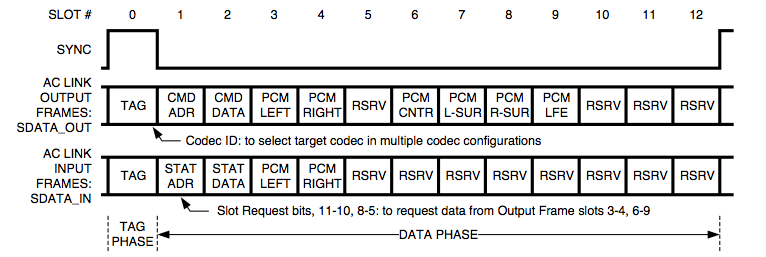
\includegraphics[scale=1]{images/LM4550_protocol.png}
					\caption{AC link bidirectional frame}
					\label{LM4550_protocol}
				\end{subfigure}
				\hfill
				\begin{subfigure}{1\textwidth}
					\centering
					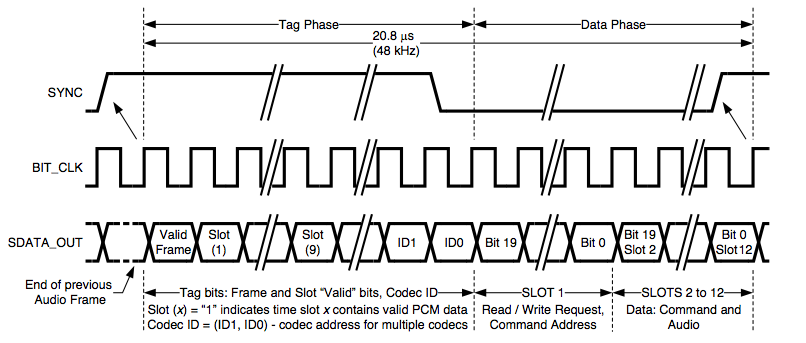
\includegraphics[scale=1]{images/LM4550_output_frame.png}
					\caption{AC link output audio frame}
					\label{LM4550_output_frame}
				\end{subfigure}
			\caption{AC link serial interface protocol}
			\end{figure}
				\item \textbf{AC97CMD command state machine:} is a state machine that creates the control data based on the inputs \texttt{snd\_eff} and \texttt{volume} and passes it to the AC97 Controller. This control data controls among others the volume of the output audio and the DAC sample rate. Figure \ref{LM4550_innen} shows the path of the audio data that gets transferred within the LM4550 chip and the registers that need to be configured along this path. The following code was extracted from the file \texttt{a97cmd\_fsm.vhd} that implements the state machine necessary to configure the registers of the LM4550 chip. It shows an example of how to activate the output \texttt{HP\_OUT}. As shown in figure \ref{LM4550_innen} \texttt{LINE\_OUT} is muted by default. 
				
				\begin{figure}[h]
					\centering
					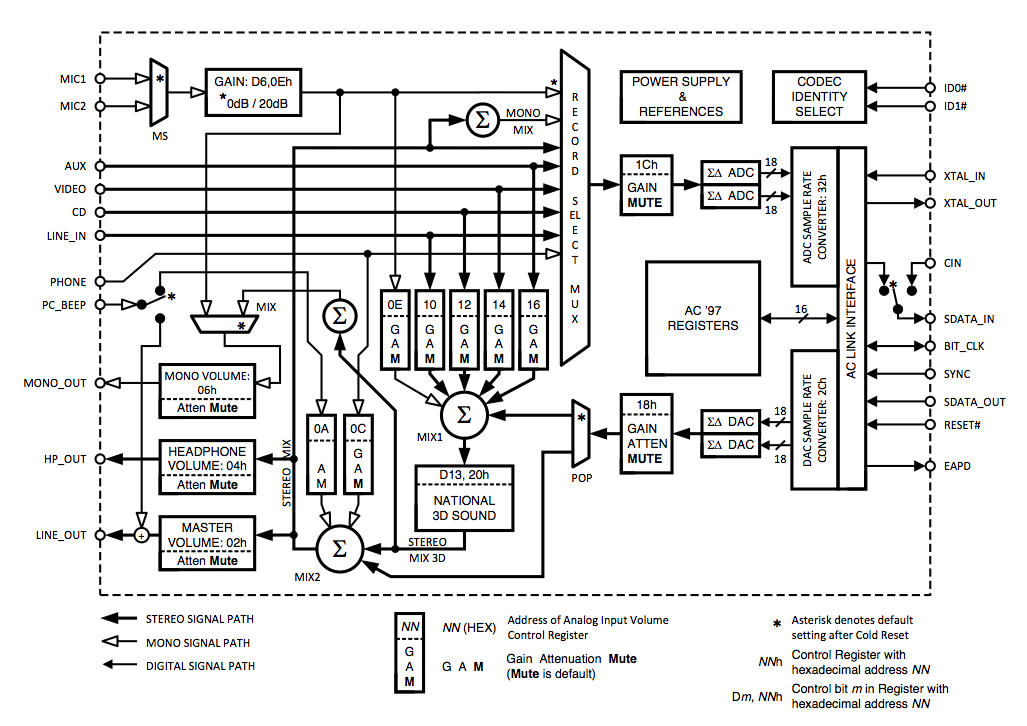
\includegraphics[scale=1]{images/LM4550_innen.png}
					\caption{Block diagram of LM4550 chip. Red line is the path from FPGA output to \texttt{HP\_OUT}. All registers along this path need to be configured.}
					\label{LM4550_innen}
				\end{figure}
\textcolor{red}{following code needs to be formatted correctly with VHDL Highlighting!}

-- -------------------------------\\
$\cdots$

process (next\_state, cur\_state, atten)\\
	begin\\

		case cur\_state is\\
			when S0 =>\\
				cmd <= X"02\_8000";  -- master volume	0 0000->0dB atten, 1 1111->46.5dB atten			\\					
				next\_state <= S2;\\
			when S1 => \\
				cmd <= X"04" \& "000" \& atten \& "000" \& atten;	-- headphone volume\\
				next\_state <= S4;\\
			when S2 => 			\\
			
			$\cdots$\\	
-- -------------------------------


The AC97CMD module also reads the audio sound effects from a ROM that gets initialized when the FPGA is programmed. The right sound effect is chosen according to the signal \texttt{snd\_eff}.
				\end{itemize}
		  
